% \section{Einfluss für den Nutzer}

In diesem Abschnitt ist festzustellen, welchen Einfluss die Lösung für den Nutzer der jeweiligen Webanwendung besitzt. Dabei gilt es bspw. den Aspekt der Ladezeit sowie des erhöhten Datenaufkommens zu beleuchten.

Um die leistungsrelevanten Daten zu erheben, wurden das Frontend jeweils ohne und mit der Lösung mithilfe des \enquote{Performance Analysis}-Werkzeugs im Firefox \cite{FirefoxPerformanceAnalysis} analysiert. Um den Aspekt der Ladezeit, also die Zeit bis die Anwendung für den Nutzer interaktiv wird, zu messen, wurde pauschal die Zeit bis zur ersten ausgehenden Datenabfrage gemessen. Die Ergebnisse sind in \autoref{fig:Einfluss-fuer-den-Nutzer_erste-Anfrage} zu betrachten. Dabei wird erkennbar, dass die Lösung eine leicht erhöhte Ladezeit aufweist - zuvor lag die durchschnittliche Ladezeit bei ~760ms und nun liegt sie bei 1080ms.

\begin{figure}[H]
	\centering
	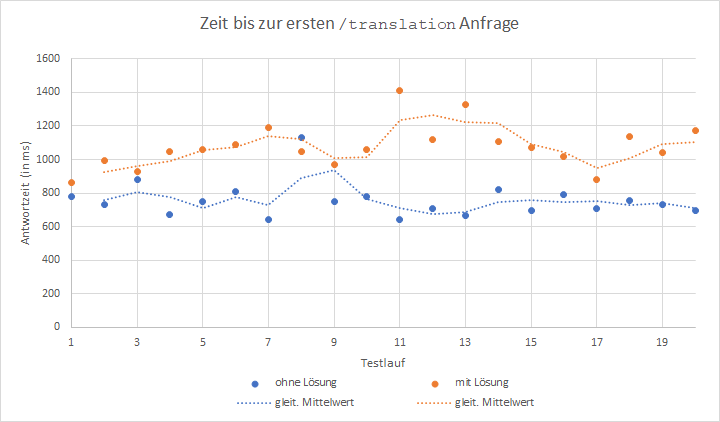
\includegraphics[width=1.00\linewidth]{data/Einfluss-fuer-den-Nutzer/Einfluss-fuer-den-Nutzer_erste-Anfrage.png}
	\caption{Einfluss für den Nutzer: Zeit bis zur ersten Anfrage}
	\label{fig:Einfluss-fuer-den-Nutzer_erste-Anfrage}
\end{figure}

Weiterhin wurde der Aspekt des erhöhten Datenaufkommens näher beleuchtet, indem pro Testlauf jeweils einmal ein Standard-Workflow in der Anwendung durchgespielt worden ist. Am Ende eines Durchlaufs wurde die Anzahl an tatsächlich\footnotemark{} übertragenden XHR-Bytes notiert, das Resultat kann in  \autoref{fig:Einfluss-fuer-den-Nutzer_gesamte-Uebertragung} betrachtet werden. Da der Nutzer selbst entscheiden kann, ob LogRocket aktiviert sein soll oder nicht, wurde die Lösung einmal mit aktivierten LogRocket und einmal deaktivierten LogRocket getestet. Weiterhin wurde die Anzahl der Anfragen notiert, vgl. \autoref{fig:Einfluss-fuer-den-Nutzer_Anzahl-Anfragen}.

Dabei lässt sich feststellen, dass das Datenaufkommen kaum erhöht ist. Grund hierfür ist, dass die zusätzlich gemeldeten Daten durch die automatisch durchgeführte Komprimierung\footnotemark{} kaum zum Datenaufkommen beitragen. Jedoch kann in der Anzahl der Anfragen eine starke Erhöhung festgestellt werden.

Letztendlich lässt sich somit feststellen, dass der Performance-Einfluss der Lösung marginal und vernachlässigbar ist.

\footnotetext{Durch Komprimierung wie gzip sind die tatsächlich zu übertragenden Bytes geringer als die eigentliche Datenmenge \cite{FirefoxContentEncoding}.}

\begin{figure}[H]
	\centering
	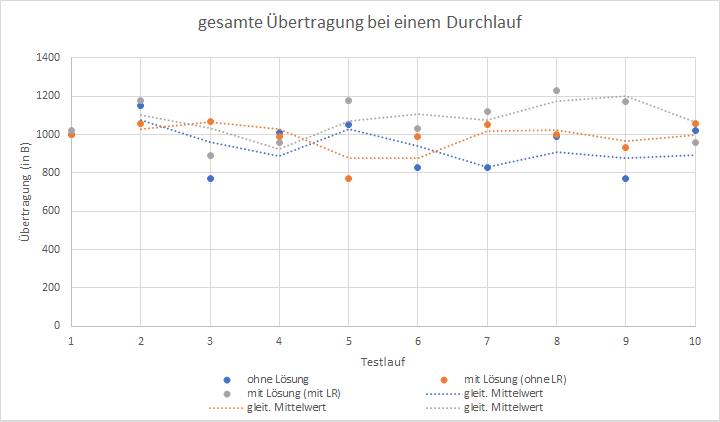
\includegraphics[width=1.00\linewidth]{data/Einfluss-fuer-den-Nutzer/Einfluss-fuer-den-Nutzer_gesamte-Uebertragung.png}
	\caption{Einfluss für den Nutzer: Gesamte Übertragungsmenge}
	\label{fig:Einfluss-fuer-den-Nutzer_gesamte-Uebertragung}
\end{figure}

\begin{figure}[H]
	\centering
	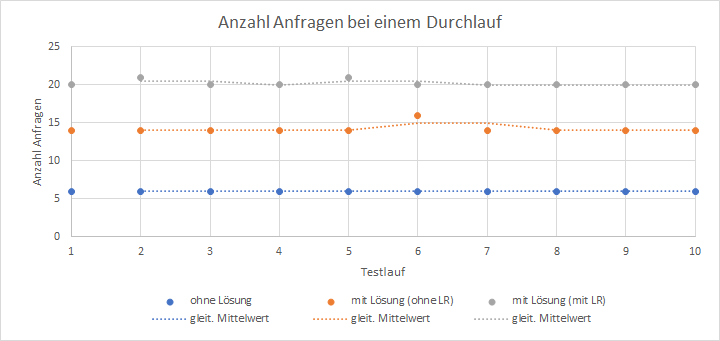
\includegraphics[width=1.00\linewidth]{data/Einfluss-fuer-den-Nutzer/Einfluss-fuer-den-Nutzer_Anzahl-Anfragen.png}
	\caption{Einfluss für den Nutzer: Anzahl der Anfragen}
	\label{fig:Einfluss-fuer-den-Nutzer_Anzahl-Anfragen}
\end{figure}
